%!TEX root=paper.tex

  \section{Automated Outlier Detection and Monitoring}
  \label{sec:outliers}
  % \va{Shouldn't this be promoted to a section? It is neither utilization- nor performance- related. Either that, or Section~\ref{sec:user} should be folded into this section too, and then Sections~\ref{sec:version} and~\ref{sec:regression} merged into another section. Otherwise we have a very scattered paper}
  
  When an API endpoint is called from within a highly interactive application (as it is the case with the case with \epTranslationsColor in the previous section) of particular interest to the API developers are performance {\em outliers}.   Indeed, a translation request that takes three times more than expected can seriously decrease the perceived quality of the application. Thus, identifying, collecting all appropriate data, and diagnosing the root causes of such outliers is especially critical in improving the quality of an application. 
  
  % In the context of the RESTful services support by Flask, this means request serving times that deviate from the average to an unexpected degree. 
  
  For this purpose the \tool tracks for every monitored endpoint a {\em running average} response time value\footnote{\ins{For performance reasons, we assume that the response times for the endpoints are normally distributed. Otherwise, more general density distribution information must be collected in real time.}}. When it detects that a given request is an outlier with respect to this past average running value, it triggers the {\em outlier data collection routine} which stores \ins{extra information} about the current execution environment. A configurable threshold with a default value of $2.5$ times the running average response time is used for this purpose. 

  For every detected outlier request, the \tool collects information about the current Python stack trace, CPU load, memory consumption, request parameters, etc. in order to allow the maintainer to investigate the causes of these exceptionally slow response times. In this way it is possible to get \ins{detailed insight into the operation of the application in the extreme cases without unnecessarily burdening it with logging this information for every request}.


  \begin{figure}[h!]
    \centering
    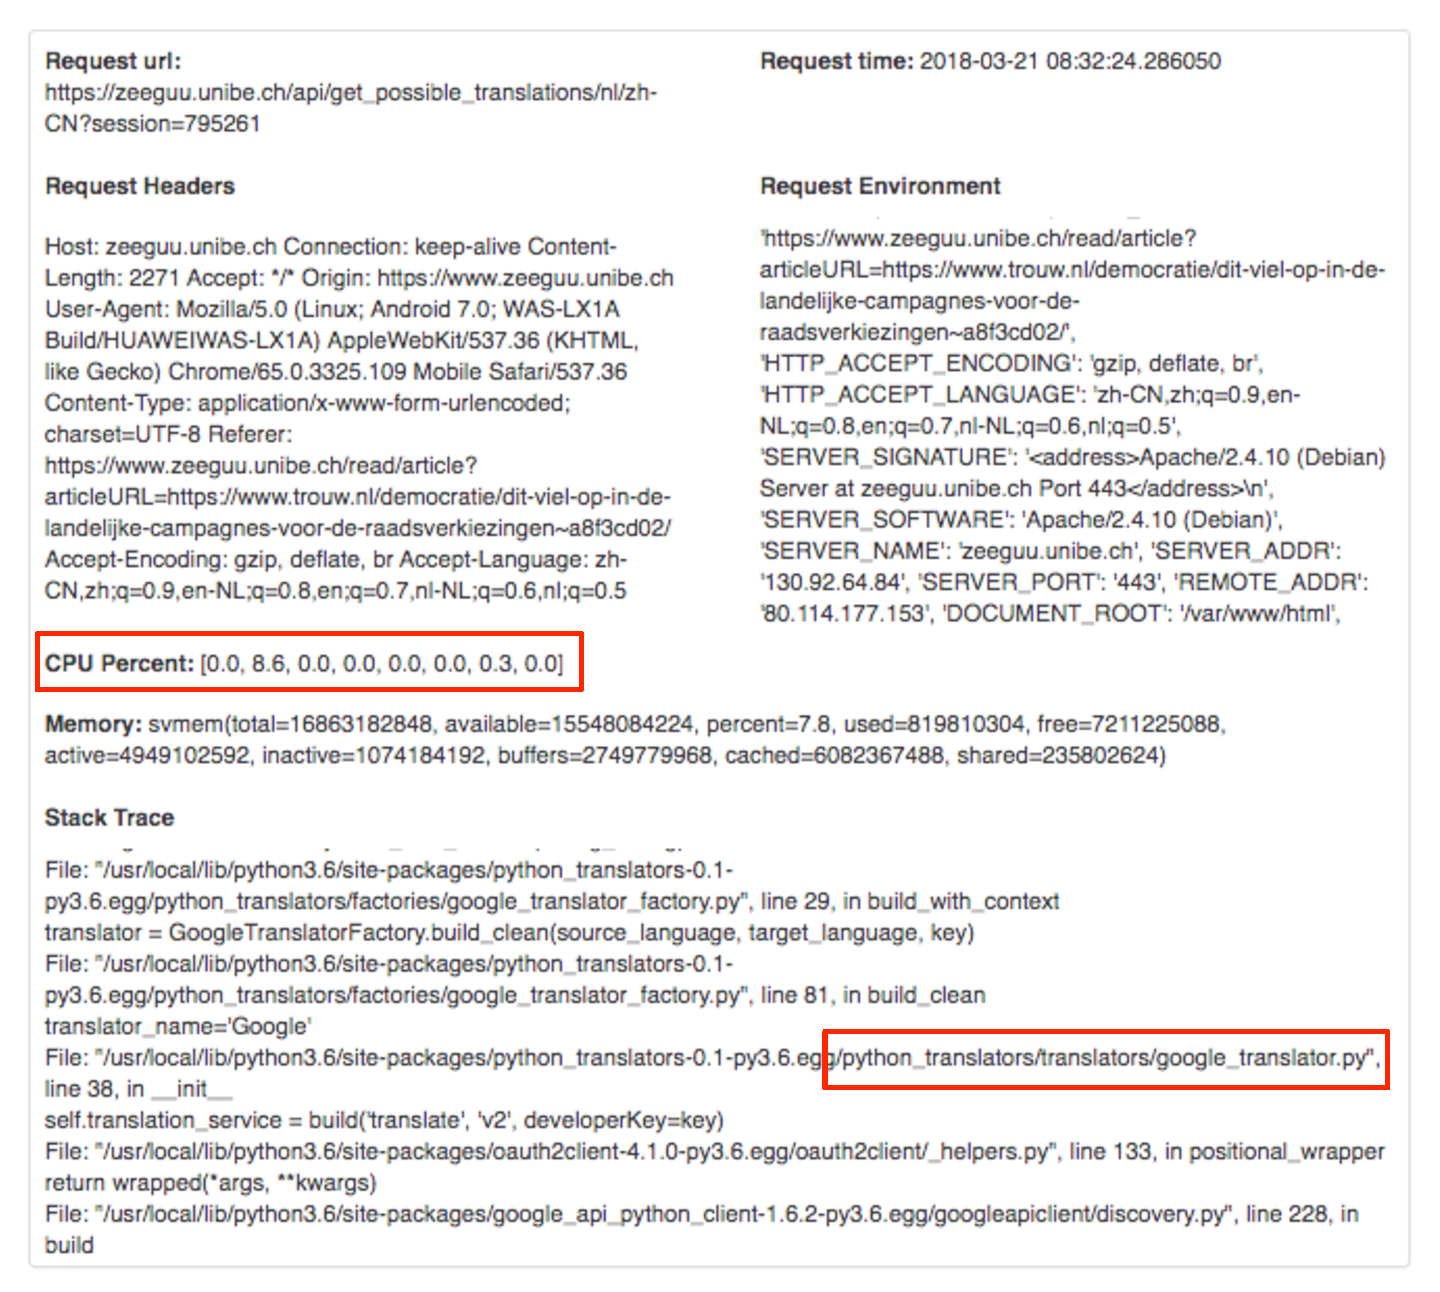
\includegraphics[width=0.9\linewidth]{outlier-annotated}
    \caption{Automatically collected outlier information}
    \label{fig:stack}
  \end{figure}
  

The bottom panel in \Fref{fig:stack} shows the stack trace. 
In this particular case, it is revealing for the developer to learn that at the time of the stack trace snapshot, the code was in the \code{google\_translator}: indeed, the system uses as back-end multiple translators, and it has been observed that many of the outliers happen while the system is waiting for the Google translator.
%
This information has to be corroborated with the observations that neither the memory nor the processor are overloaded at the moment. Thus this functionality in \code{microsoft\_translator} is really slow in itself, and this is not a result of the machine being overloaded for example. \va{last sentence does not parse}




